\documentclass[a4paper, fontsize=14pt]{article}
\usepackage{scrextend}
\usepackage{indentfirst, fancyhdr, amsfonts, mathtools, amssymb}
\usepackage{titlesec} %работа с рубрикацией
\usepackage{tocloft} %настройки оглавления
\usepackage[T2A]{fontenc}
\usepackage[utf8x]{inputenc}
\usepackage[russian]{babel}
\usepackage{hyperref} %кликабельное оглавление
\usepackage[left=3.7cm,right=2cm,top=2cm,bottom=2cm]{geometry}
\usepackage{tempora} %настраиваем шрифт типа TNR                                   
\usepackage{newtxmath} %делаем шрифт формул похожим на TNR
\usepackage{caption}
\usepackage{listings}
\lstset{
  columns=fullflexible,
  breaklines=true,
}
\linespread{1}
\setcounter{page}{4} %в зависимости от того, какой по счёту страницей должно быть оглавление!

%НАСТРОЙКИ ОГЛАВЛЕНИЯ
\renewcommand{\cftsecaftersnum}{.} %точки после номеров разделов и подразделов в оглавлении
\renewcommand{\cftsubsecaftersnum}{.}
\renewcommand{\cftsecfont}{\normalfont} %разделы в оглавлении пишутся обычным (не жирным) шрифтом
\renewcommand{\cftsecpagefont}{\normalfont} %соответствующие им страницы тоже
\renewcommand{\cftsecleader}{\cftdotfill{\cftdotsep}} %расставляем точки между названиями разделов и их страницами
\addto\captionsrussian{\renewcommand\contentsname{СОДЕРЖАНИЕ}} %хотим, чтобы слово "Содержание" писалось капсом
\renewcommand{\cfttoctitlefont}{\hfil\bfseries} %слово СОДЕРЖАНИЕ по центру жирным
\renewcommand{\cftaftertoctitle}{\hfill}

%НАСТРОЙКИ РУБРИКАЦИИ
\titleformat*{\section}{\center\bf} %названия разделов и подразделов по середине жирным шрифтом
\titleformat*{\subsection}{\center\bf}
\titlelabel{\thetitle.\quad} %название раздела и его номер отделены точкой

%НАСТРОЙКИ БИБЛИОГРАФИИ
\addto\captionsrussian{\renewcommand\refname{СПИСОК ЛИТЕРАТУРЫ}} %хотим, чтобы слова "Список литературы" писались капсом
\makeatletter
\renewcommand{\@biblabel}[1]{#1.} %хотим, чтобы в списке литературы номера источников писались в формате "No. <...>", а не "[No] <...>"
\makeatother

\begin{document}
\textbf{Цель работы:}  Получить навык проведения вычислительного эксперимента, направленного на решение задач интерполирования и аппроксимации функций.
\subsection*{{Ход работы}}
\subsubsection*{Задача №1}
\begin{enumerate}
   \item	Написать вычислительную программу на языке программирования C++ для построения интерполяционного многочлена Лагранжа $L_n(x)$ произвольной степени $n$ по известным значениям функции $y_i=f(x_i)$, заданным на сетке узлов $a=x_0<x_1<…<x_{n-1}<x_n=b.$
   \item Для каждого $n=1,\dots,15$ построить интерполяционный многочлен Лагранжа $L_n(x)$ по значениям функции на равномерной сетке узлов:
           \begin{equation}
            \label{uniform_grid}
            x_i+1 =x_i+h, \quad  x_0=a,  \quad  h=\frac{b-a}{n}
           \end{equation}
             и найти оценку погрешности приближения функции  
             \begin{equation}
                \label{delta}
                \Delta_n=sup|f(x)-L_n(x)|,  \quad  x \in [a,b].
             \end{equation}
   Оценку $\Delta_n$ провести численно посредством вычисления модуля ошибки приближений $|f(x)-Ln(x)|$ в узлах мелкой равномерной сетки, состоящей из $~10^5$ узлов, с выбором максимального значения в качестве искомой оценки.    
   \item	Построить график зависимости $\Delta_n$ от $n$ определить оптимальную степень $n_0$, при которой погрешность минимальна. 
\item	Построить график ошибки приближения $f(x)-L_{n_0}(x)$.
\end{enumerate}
\subsubsection*{Решение}
Задана функция:
\begin{equation}
    \label{target_f}
    f(x) = \frac{\operatorname{arctg}(x)}{1+x^2}
\end{equation}

Необходимо построить интерполяционный многочлен в виде:
\begin{equation*}
    L_n(x) = \sum_{i=1}^n f(x_i) \prod_{j \neq i} \frac{x-x_j}{x_i-x_j}
\end{equation*} 

Соответствующий код расчета многочлена в точке $x_0$ приведен в приложении.

Согласно заданию, построим многочлены Лагранжа степеней $n=1,\dots,15$ для функции \eqref{target_f} на равномерной сетке \eqref{uniform_grid} и численно найдем оценку погрешности \eqref{delta}. Данные запишем в Таблицу 1.
\begin{center}
    \begin{tabular}{|c | c |} 
     \hline
     $n$ & $\Delta_n $\\ \hline 
     1    &   1.776300\\ \hline
     2    &   0.562909\\ \hline
     3    &   0.439082\\ \hline
     4    &   0.114664\\ \hline
     5    &   0.083134\\ \hline
     6    &   0.105621\\ \hline
     7    &   0.050630\\ \hline
     8    &   0.002494\\ \hline
     9    &   0.014350\\ \hline
     10   &   0.011087\\ \hline
     11   &   0.003506\\ \hline
     12   &   0.000860\\ \hline
     13   &   0.001649\\ \hline
     14   &   0.000901\\ \hline
     15   &   0.000147\\ \hline
    \end{tabular}
    \label{Table:errorofLagrange}
    \captionof{table}{Зависимость $\Delta_n$ от $n$}
    \end{center}

    Таким образом, видно, что наилучшим образом функцию \eqref{target_f} приближает многочлен степени $n_0=15$ c $\Delta_{15} = 1.47 10^-4$. 
    
    График ошибки $| f(x)-L_{n_{15}}(x) |$ представлен на рисунке 1.
    
    \begin{center}
        \label{delta_15}
        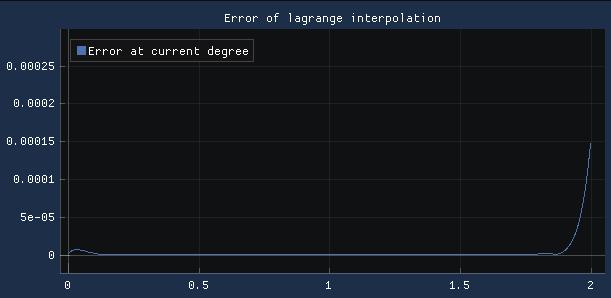
\includegraphics[]{src/lagrange_n_15_error.png}
        \captionof{figure}{График зависимости $\Delta_n$ от $x$ в узхлах тестовой равномерной сетки}
    \end{center}
    
    Сильный всплеск на конце обусловлен тем, что концевая точка не является узлом интерполяционной сетки. Точки интерполяции продемонстрированы на рисунке 2.. Расхождение функций $L_{15(x)}$ и $f(x)$ в окрестности точки $a = 2$ видно на риснуке 3.
    \begin{center}
        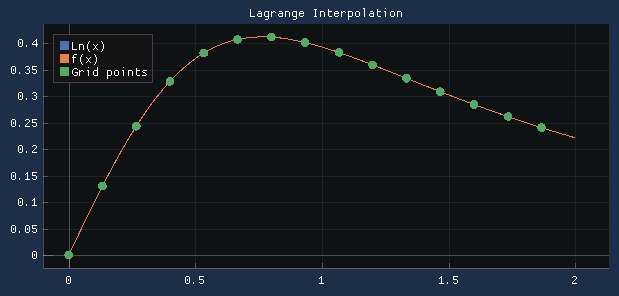
\includegraphics[]{src/lagrange_n_15.png}
        \captionof{figure}{Графики $L_{15}(x)$ и $f(x)$ с указанием узлов интерполяции}
    \end{center}

    \begin{center}
        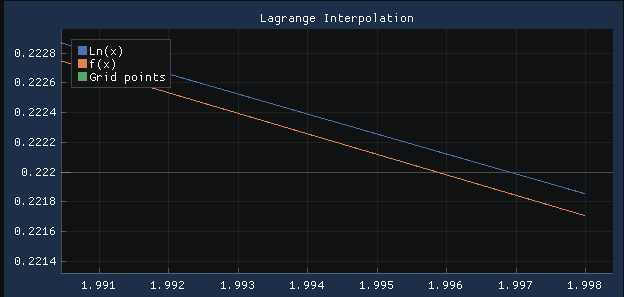
\includegraphics[]{src/lagrange_error_at_the_end.png}
        \captionof{figure}{Расхождение функций $L_{15(x)}$ и $f(x)$  на конце отрезка}
    \end{center}

    \subsubsection*{Задача №2}
    \begin{enumerate}
        \item Построить сетку узлов, составленных из нулей многочлена Чебышева степени $n_0$, найденной при решении предыдущей задачи:
        \begin{equation}
            \label{chebyshev_roots}
            x_i=\frac{b+a}{2} + \frac{b+a}{2}  \cos \left(\frac{\pi (2i+1)}{2 n_0 }\right),  \quad  i=0,1,\dots,n_{0}-1.
        \end{equation}
        
        Найти численные значения заданной функции \eqref{target_f} в этих узлах: $$y_i=f(x_i)$$
        \item  С использованием написанной при решении Задачи 1 программы построить по этим данным многочлен Лагранжа $L_{n_0}(x)$ степени $n_0$.
        \item  Найти оценку погрешности приближения функции $\Delta_{n_0}$ и сравнить ее с известной теоретической минимальной оценкой погрешности интерполяции многочленом Лагранжа.
        \item  Выполнить сравнение двух многочленов Лагранжа $L_{n_0}(x)$ на равномерной и неравномерной сетках, построенных в этой и предыдущей задачах.
    \end{enumerate}
    \subsubsection*{Решение}
    Вычисление корней $x_i$ многочлена Чебышева \eqref{chebyshev_roots} и соответствующих значений $y_i$ в приведено в приложении. Узлы интерполяции, построенный по ним интерполяционный многолчен Лагранжа $L_{15}$ и фукнция \eqref{target_f} продемонстрированы на рисунке 4. 
    \begin{center}
        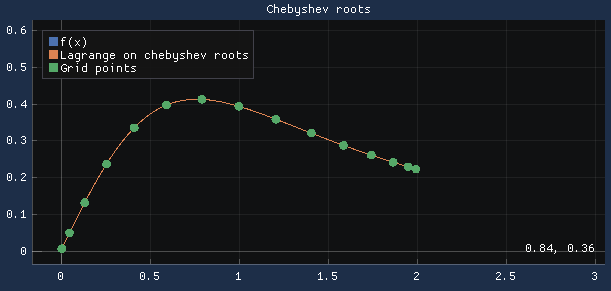
\includegraphics[]{src/chebyshev_roots.png}
        \captionof{figure}{Графики $L_{15}(x)$ и $f(x)$ с указанием узлов интерполяции на чебышевской сетке}
    \end{center}
    

    Как видно из рисунка 4 на концах отрезка узлы интерполяции расположены более плотно, чем в середине отрезка. 

    При этом оценка \eqref{delta} составляет $\Delta_{15} = 3,451 \cdot 10^{-7}$, что на  три порядка ниже, чем на равномерной сетке.
    
    При чебышевских узлах интерполирования теоретическая оценка принимает вид:
    \begin{equation}
        \label{chebyshev_estimate}
        || f(x) - L_n(x) || \leq \frac{|| f^{(n)}(x) ||}{n!} 2^{1-2n} (b-a)^n
    \end{equation}

    С использованием пакета Maple вычислим оценку \eqref{chebyshev_estimate}. Листинг программы приведен в приложении.
    Получим, что:
    \begin{equation*}
        || f(x) - L_n(x) || \leq 8,242 \cdot 10^{-6}
    \end{equation*}
    Что согласуется c полученным выше численным расчетом.
    \subsubsection*{Задача №3}
    \begin{enumerate}
        \item Написать вычислительную программу на языке программирования C++ для построения интерполяционного многочлена Ньютона порядка $n_0$ (найдено при решении Задачи 1) на равномерной сетке через вычисление разделенных разностей.
        \item Выполнить сравнение построенного многочлена Ньютона с аналогичным многочленом Лагранжа, построенного при решении первой задачи.
    \end{enumerate}
    \subsubsection*{Решение}
    Требуется построить интерполяционный многочлен для фукнции \eqref{target_f} в виде:
    \begin{equation*}
        L_n = f(x_0) + \sum_{k=1}^{n+1} \prod_{i=0}^{k-1} (x-x_i) f(x_0; \dots; x_k)
    \end{equation*}
    Здесь $f(x_0; \dots;x_k)$ разделенная разность, вычисляющаяся по формуле:
    \begin{equation*}
        f(x_0; \dots;x_k) = \frac{f(x_0; \dots;x_{k-1}) - f(x_1; \dots;x_k)}{x_0 - x_k}
    \end{equation*}

    Код расчета приведен в приложении.

    Интерполяция данным методом дает ошибку больше, чем при интерполяции в форме Лагранжа, однако работает в среденем гораздо быстрее за счет уменьшения колличества операций.
    В данной конкретной реализации при $n=15$ оценка ошибки начала различаться в $12$ знаке мантиссы. 
    Кроме того, в форме Ньютона можно добавлять узлы интерполяции лишь просчитав разделенную разность и добавив её к общей сумме, в то время как многочлен Лагранжа пришлось бы пересчитывать заново.

    \subsubsection*{Задача №4}
    \begin{enumerate}
        \item Написать вычислительную программу на языке программирования С++, осуществляющую интерполяцию функции $g(t), t\in[0,2\pi]$, заданной своими значениями $g(t_i) (i=1,\dots,2n+1)$ в узлах $$t_i=2 \pi (i-1)/(2n+1)$$ равномерной сетки, тригонометрическим многочленом $F_n(x)$:
        \begin{equation*}
            F_n(t)=\frac{a_0}{2}+\sum_{k=1}^{n} \left( a_k  \cos(kt)+b_k \sin(kt) \right)
        \end{equation*}
        \item Построить линейную замену переменных $x=\alpha t+ \beta$, переводящую заданный отрезок $[a,b]$ в отрезок $[0,2\pi]$. Выполнить эту замену переменных в аргументе функции $f(x): f(\alpha t+\beta) = g(t)$.
        \item С использованием написанной программы провести вычислительный эксперимент по нахождению минимальной степени $m$ тригонометрического многочлена, обеспечивающего приближение функции с указанным в задании предельным уровнем погрешности $\delta = 10^{-3}$:
        \begin{equation*}
            \operatorname{sup} |g(t)-F_m (t)| \leq \delta.
        \end{equation*}
        \item Оценку погрешности производить по способу, описанному в Задаче 1. Построить график ошибки приближения функции многочленом.
    \end{enumerate}
    
    \subsubsection*{Решение}
    Код расчета и линейной замены приведен в приложении.

    Проведя вычислительный эксперимент, не была получена желаемая оценка погрешности $\delta$. Наилучший результат при степени многолчена $n=100$ составлял $\delta_{100} = 0,00147..$. Это связано с тем, что функция \eqref{target_f} не является периодической на отрезке $[a, b]$. Следовательно, для неё не выполнена теорема Дирихле о разложении в тригонометрический ряд Фурье. А значит, мы никогда не сможем добиться желаемого результата.
    \begin{center}
        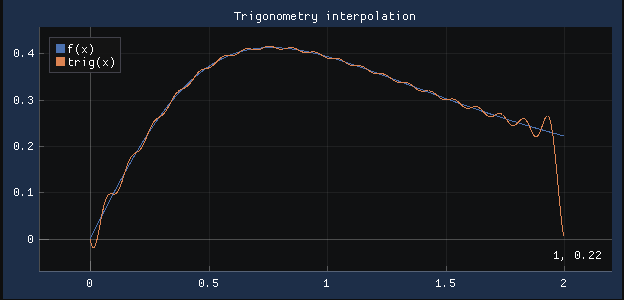
\includegraphics[]{src/trig_plot.png}
        \captionof{figure}{Графики $F_n(x)$ и $f(x)$ на равномерной сетке}
    \end{center}
    
    Из рисунка 5 видно, что тригонометрическая интерполяция на концах отрезка дает ощутимый вклад в ошибку $\Delta$.
    График соответствующей оценки приведен на рисунке 6.

    \begin{center}
        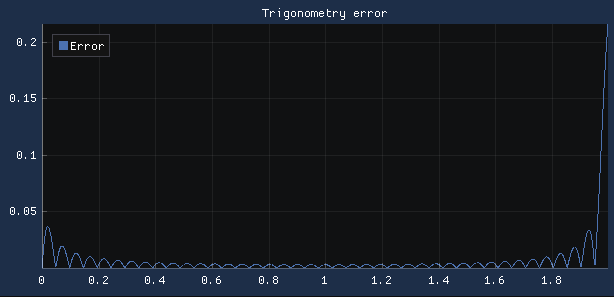
\includegraphics[]{src/trig_error.png}
        \captionof{figure}{График ошибки функции $F_n(x)$ на равномерной сетке}
    \end{center}
    \subsubsection*{Задача №5}
    \begin{enumerate}
        \item Написать вычислительную программу на языке С++, позволяющую построить многочлен наилучшего равномерного приближения $Q_n$ степени $n$ для произвольного многочлена $P_{n+1}$ степени $n+1$.
        \item С использованием математического пакета (Maple или MATLAB) выполнить разложение заданной функции $f(x)$ в ряд Тейлора в окрестности точки $\frac{a+b}{2}$ и определить степень $n$, при которой соответствующий многочлен $P_n(x)$, представляющий собой отрезок ряда Тейлора, приближает функцию $f(x)$ с указанным в задании предельным уровнем погрешности $\delta = 10^{-3}$:
        \begin{equation*}
            f(x) \approx P_n (x)=\sum_{k=0}^n b_k x^k,  \quad    \operatorname{sup} |f(x)-P_n (x)| \leq \delta
        \end{equation*}
        \item 	С использованием написанной программы телескопическим методом построить многочлен $Q_m$ наилучшего равномерного приближения наименьшей степени $m$, обеспечивающий приближении исходной функции $f(x)$ с той же точностью:
        \begin{equation*}
            \operatorname{sup} |f(x)-Q_m (x)| \leq \delta
        \end{equation*}
        Построить график ошибки приближения функции многочленом $Q_m$.
        
    \end{enumerate}
    \subsubsection*{Решение}

    Заметим, что для любого интеполяционного многочлена справедливо:
    \begin{equation*}
        || f(x) - Q_n(x) || = \operatorname{sup} | f(x) - Q_n(x) | \geq \operatorname{min}|f^{(n+1) (x)} | \cdot \frac{\operatorname{max}|\omega_{n+1}(x)|}{(n+1)!}
    \end{equation*}
    где максимум и минимум берутся по отрезку $[a, b]$.
    Наилучшая оценка достигается при чебышевских узлах интерполяции:
    \begin{equation}
        \label{mnrp_est1}
        || f(x) - Q_n(x) || \geq \operatorname{min}|f^{(n+1) (x)} | \cdot \frac{(b-a)^{n+1}}{2^{2n+1} (n+1)!}
    \end{equation}
    Теперь оценим сверху. Так как $Q_n$ есть МНРП, то $||f - Q_n || \leq || f - P_n ||$, где $P_n$ любой многочлен степени $n$. Пусть $P_n = L_n$, то есть интерполяционный многочлен с чебышевскими узлами. Тогда:
    \begin{equation*}
        | f(x) - Q_n(x) | \leq \operatorname{max} |f^{(n+1)(x)}| \cdot \frac{(b-a)^{n+1}}{2^{2n+1} (n+1)!}
    \end{equation*}

    То есть получаем, что:
    \begin{equation}
        \label{mnrp_est2}
        || f(x) - Q_n(x) || \leq || f - L_n || \leq \operatorname{max} |f^{(n+1)(x)}| \cdot \frac{(b-a)^{n+1}}{2^{2n+1} (n+1)!}
    \end{equation}

    То есть, применяя теорему о двух жандармах к уравнениям \eqref{mnrp_est1} и \eqref{mnrp_est2}, получаем, что МНРП $Q_n$ должен быть интерполяционным многочленом с чебышевскими узлами.

    Таким образом, первый пункт Задачи 5 сводится к Задаче 2. Соответствущий код приведен в приложении.

    Теперь аппроксимируем функцию \eqref{target_f} рядом Тейлора. С помощью пакета Maple найдем, что нужна оценка $\delta = 10^-3$ достигается при степени разложения $n=20$. Код расчетов приведен в приложении. 

    Телескопическим методом, начиная от $n=20$ найдем степень, при которой МНРП меньшей степени будет оптимальным. Код расчетов прикреплен в приложении. 
    
    Получим, что оптимальным будет являться многочлен степени $n=9$.
    На рисунке 7 продемонстрирован график ошибки $\Delta_9(x) = | f(x) - Q_9(x) |$.
    \begin{center}
        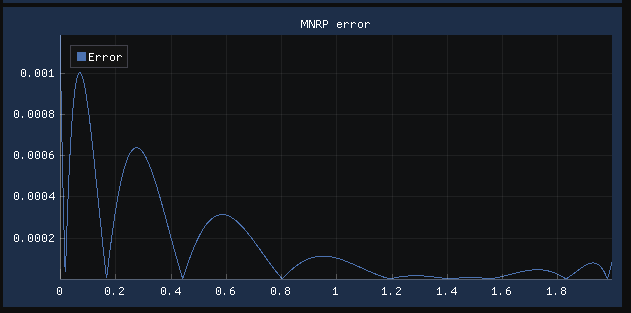
\includegraphics[]{src/mnrp_error.png}
        \captionof{figure}{График $\Delta_9$(x)}
    \end{center}
    \subsubsection*{Задача 6}
    \begin{enumerate}
        \item Написать вычислительную программу на языке программирования C++ для построения интерполирующего кубического сплайна по значениям функции, известным в узлах равномерной сетки. 
        \item С использованием написанной программы провести вычислительный эксперимент по определению минимального количества узлов равномерной сетки, обеспечивающих построение интерполирующего сплайна для заданной функции с указанным в задании предельным уровнем погрешности. Погрешность интерполяции оценивать способом, описанным в Задаче 1.
        \item Построить график ошибки приближения заданной функции интерполирующим сплайном.
    \end{enumerate}
    
    \subsubsection*{Решение}

    Код расчетов приведен в приложении. 

    Были получены следующие результаты: необходимое количество сплайнов равно $n=8$, при этом $\Delta = 8,949 \cdot 10^{-4}$. График ошибки приведен на рисунке 8.

    \begin{center}
        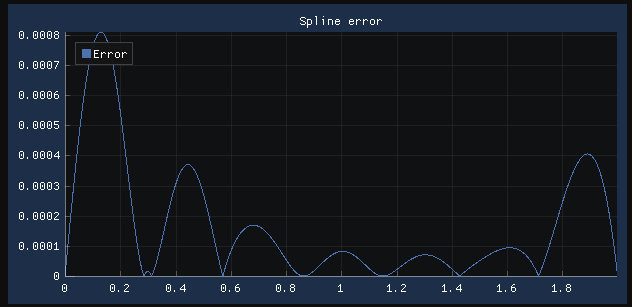
\includegraphics[]{src/spline_error.png}
        \captionof{figure}{График ошибки $\Delta$ при восьми сплайнах}
    \end{center}
    \newpage
\section*{{Вывод}}

\newpage
\section*{{Приложение}}

Весь код выложен в репозитории: ....
% \begin{thebibliography}{5}
% \end{thebibiliography}

Расчет теоретической оценки для интерполяции на чебышевской сетке
\begin{figure*}[h!]
    \begin{verbatim}
with(Optimization):
f:=(arctan(x) / (1 + x^2)):
f_prime := diff(f, x$15):
fn := Maximize(f_prime, x=0..2)[1]:
evalf(fn / 15! * 2^(1-30) * 2^15);
    \end{verbatim}
\end{figure*}


Расчет наилучшей степени разложения ряда Тейлора
\begin{figure*}[h!]
    \begin{verbatim}
f := arctan(x)/(x^2 + 1);
a := 0;
b := 2;

epsilon = evalf(10^(-3));
q := taylor(f, x = (a + b)/2, 20);
p := convert(q, polynom);
p := evalf(simplify(p));
delta := 0;
for i to 100 do x[i] := evalf(a + i*(b - a)/100); y[i] := evalf(subs(x = x[i], f)); pn[i] := evalf(subs(x = x[i], p)); d[i] := abs(y[i] - pn[i]); if delta < d[i] then delta := d[i]; end if; end do;
delta;

q := evalf(series(f, x = (a + b)/2, 20));
    \end{verbatim}
\end{figure*}

\end{document}